\documentclass{beamer}
%
% Choose how your presentation looks.
%
% For more themes, color themes and font themes, see:
% http://deic.uab.es/~iblanes/beamer_gallery/index_by_theme.html
%
\mode<presentation>
{
  \usetheme{Madrid}      % or try Darmstadt, Madrid, Warsaw, ...
  \usecolortheme{beaver} % or try albatross, beaver, crane, ...
  \usefonttheme{serif}  % or try serif, structurebold, ...
  \setbeamertemplate{navigation symbols}{}
  \setbeamertemplate{caption}[numbered]
} 

\usepackage[english]{babel}
\usepackage[utf8x]{inputenc}
\usepackage{xcolor}
\usepackage{listings}
\usepackage{algorithm2e}
\usepackage{graphicx}
\lstset
{
    language=[LaTeX]TeX,
    breaklines=true,
    basicstyle=\tt\scriptsize,
    %commentstyle=\color{green}
    keywordstyle=\color{blue},
    %stringstyle=\color{black}
    identifierstyle=\color{magenta},
}

\title[CS396]{Auto Scaling of Key Value stores}
\author{Raghukul Raman}
\institute{IIT Kanpur}
\date{\today}

\AtBeginSection[]
{
  \begin{frame}<beamer>
    \frametitle{Outline}
    \tableofcontents[currentsection,currentsubsection]
  \end{frame}
}

\begin{document}

\begin{frame}
  \titlepage
\end{frame}

% Uncomment these lines for an automatically generated outline.
\begin{frame}{Outline}
  \tableofcontents
\end{frame}

\section{Abstract}

\begin{frame}{Aim}
    \begin{itemize}
        \item design a system to collect real time statistics on cluster based system.
        \item Collect statistics for different queries on different scaling configurations
            and try to find possible bottlenecks in the system.
        \item Providing an auto-scaling solution for key
                value stores. 
    \end{itemize}
\end{frame}

\section{Introduction}


\begin{frame}{Key Value Stores}
    \begin{itemize}
        \item Data is organized in just 2 columns - a \textbf{key}, and a \textbf{value}.
        \pause
        \item Actual data is value - can be object, keys are used to index these data objects.
        \pause
        \item Satisfy \textbf{BASE} property.
            \pause
            \begin{itemize}
                \item Basically Available
                \pause
                \item Soft state
                \pause
                \item Eventually consistent
            \end{itemize}
        \pause
        \item \textbf{CAP} theorem
            \begin{itemize}
                \pause
                \item Consistency
                \pause
                \item Availability
                \pause
                \item Partition tolerance
            \end{itemize}
       \pause
        \item Fall into CP category.
        \pause
        \item Mostly In-memory - extremy fast compared to traditional DBs.
    \end{itemize}
\end{frame}

\begin{frame}{Scalability}
    \begin{itemize}
        \pause
        \item \textit{def:} Property of a system to handle a growing amount of work by adding resources
            to the system[Bondi, Andre - 2000].
        \pause
        \item Two variants:
            \begin{itemize}
                \pause
                \item \textbf{Vertical Scaling:} Increasing the resources in the
                        server which we are currently using, i.e increase the amount of memory, CPU etc.
                \pause
                \item \textbf{Horizontal Scaling:} Increasing the number of servers (instances).
            \end{itemize}
        \pause
        \item Benefits of horizontal scaling:
            \begin{itemize}
                \pause
                \item make system fault tolerant.
                \pause
                \item down time.
            \end{itemize}
        \pause
        \item Several load balancing schemes are used in horizontal scaling.
    \end{itemize}
\end{frame}


\begin{frame}{Auto Scaling}
\begin{itemize}
    \pause
    \item Implemented in four phases of MAPE loop:
        \begin{itemize}
            \pause
            \item Monitoring
            \pause\item Analysis
            \pause\item Planning
            \pause\item Execution
        \end{itemize}
    \pause\item In this project we aim to work on the monitor and analysis phase.
    \pause\item Why AutoScaling?
        \begin{itemize}
            \pause\item To prevent overprovisioning.
        \end{itemize}
\end{itemize}
\end{frame}


\begin{frame}{Redis}
    \begin{itemize}
        \pause\item developed by Salvatore Sanfilippo(\textit{antirez}).
        \pause\item Open source, in-memory data structure store, used as a database, cache and message broker.
        \pause\item Supports other data structures like: strings, hashes, lists, sets, sorted sets with range queries, bitmaps, hyperloglogs.
        \pause\item Built in support for replication, on-disk persistance and automated partitioning with Redis cluster.
        \pause\item Master-slave asynchronous replication.
        \pause\item Transaction, expiration time (BigTable).
    \end{itemize}
\end{frame}

\begin{frame}{Redis Cluster}
    \begin{itemize}
        \pause\item Collection of redis nodes
            \begin{itemize}
                \pause\item Able to communicate among themselves.
                \pause\item Able to respond to requests collectively.
            \end{itemize}
        \pause\item Data is automatically sharded across multiple Redis nodes.
        \pause\item Every redis node require 2 ports:
            \begin{itemize}
                \pause\item Lower one is used to server clients.
                \pause\item Other used for Cluster Bus (node-to-node communication).
            \end{itemize}
        \pause\item CRC16 hashing system - $16384$ hash slots.
        \pause\item Each cluster node is responsible for a subset of hash slots.
        \pause\item Hash tags.
        \pause\item After cluster meet, every node contain node - hash slot mapping.
    \end{itemize}
\end{frame}

\begin{frame}{Resharding}
\begin{itemize}
    \pause\item Redis Cluster supports the ability to add and remove nodes while the cluster is running.
    \pause\item Same basic mechanism can be used in order to rebalance the cluster, add or remove nodes.
    \pause\item Moving hash slots through Cluster Bus.
    \pause\item No down time - with the help of MOVED Error.
\end{itemize}
\end{frame}

\begin{frame}{Redirection}
\begin{itemize}
    \pause\item Client knows nothing - can send request to any node.
    \pause\item On recieving a request:
        \begin{itemize}
            \pause\item return the value if serves that hash slot.
            \pause\item MOVED error, if not served.
        \end{itemize}
    \pause\item MOVED error response also contain IP:PORT of node serving that hash slot.
    \pause\item Still is an overhead.
\end{itemize}
\end{frame}


\begin{frame}{Partioning}
\begin{itemize}
    \pause\item The way how we shard data among different nodes of redis cluster.
    \pause\item \textbf{Client side partitioning:} redis clients select the node to which read/write request need to be made.
    \pause\item \textbf{Proxy assisted partitioning:} client sends request to a proxy,
        which analyzes the request and forwards it to the correct node.
    \pause\item \textbf{Query Routing:} can send request to any node, and the node
        will forward our request to the desired correct node.
    \pause\item Examples: Jedis, twemproxy, Redis Cluster. 
\end{itemize}
\end{frame}

\begin{frame}{Twemproxy}
\begin{itemize}
    \pause\item Proxy assisted partitioning implementation.
    \pause\item It maintains \textbf{persistent} server connections.
    \pause\item Shard data automatically across multiple servers, keeps copy of node configurations.
    \pause\item Not a single point of failure.
    \pause\item Stats monitoring port.
\end{itemize}
\end{frame}

% Introduction section ends here.
\section{Experiments}

\begin{frame}{Experiments}
\begin{itemize}
    \pause\item Collecting stats - by limiting resources.
    \pause\item Generate random strings of length 64 - mimic SHA2.
    \pause\item Tests based on get/set commands.
    \pause\item Resource limitation enforced using docker.
\end{itemize}
\end{frame}


\begin{frame}
    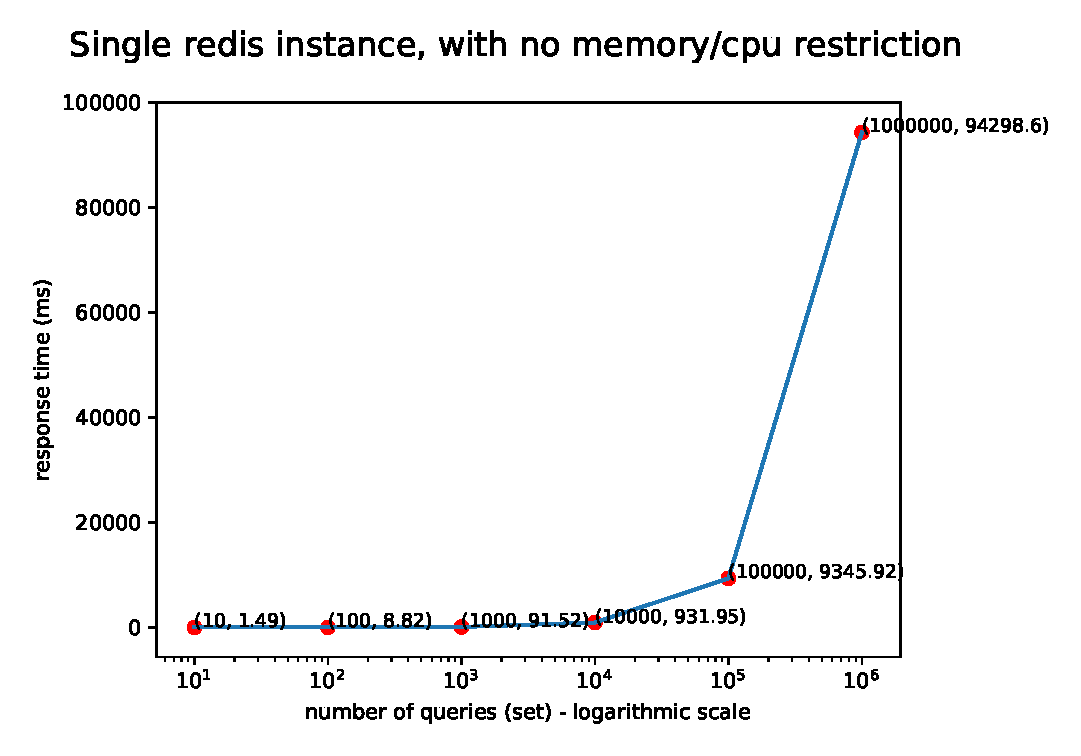
\includegraphics[width=\textwidth]{fig1.eps}
\end{frame}


\begin{frame}
    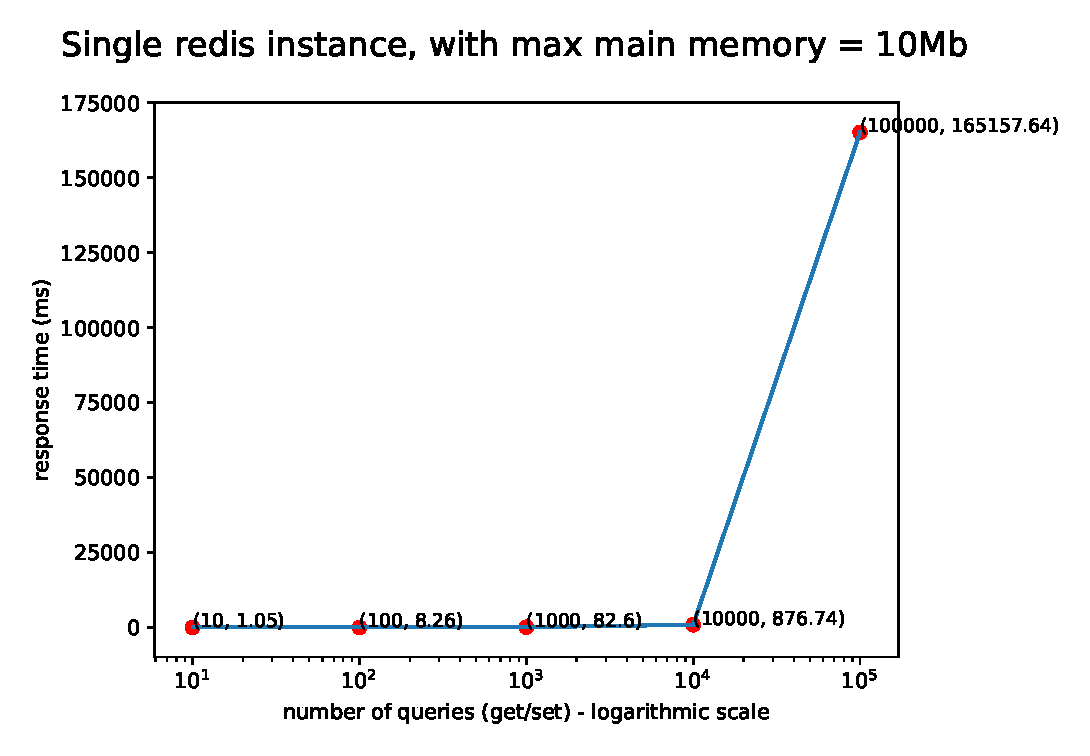
\includegraphics[width=\textwidth]{fig2.eps}
\end{frame}


\begin{frame}
    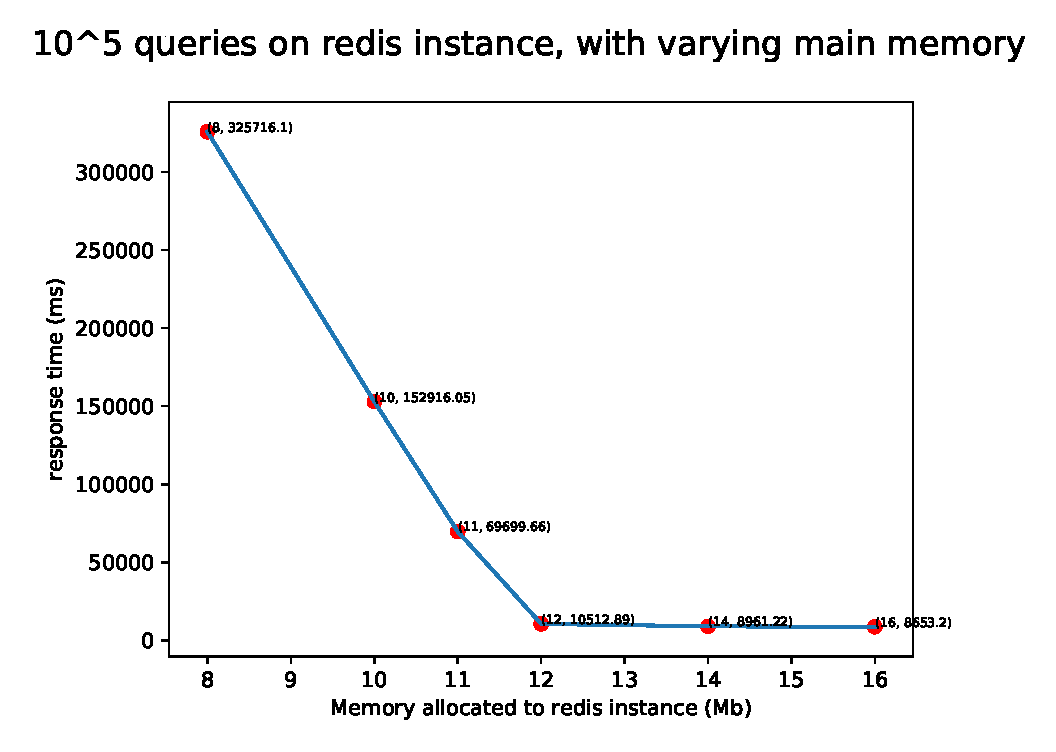
\includegraphics[width=\textwidth]{fig3.eps}
\end{frame}

\begin{frame}
\begin{center}
    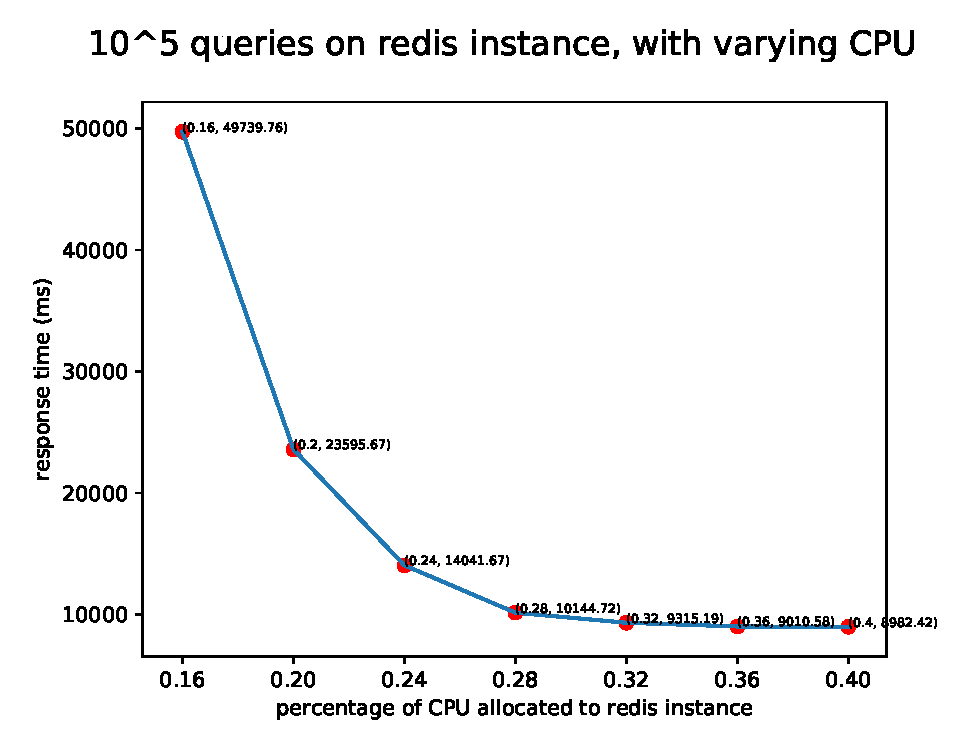
\includegraphics[width=0.8\textwidth]{fig4.eps}
\end{center}
    \begin{itemize}
        \pause\item fractional CPUs?
    \end{itemize}
\end{frame}

\begin{frame}
    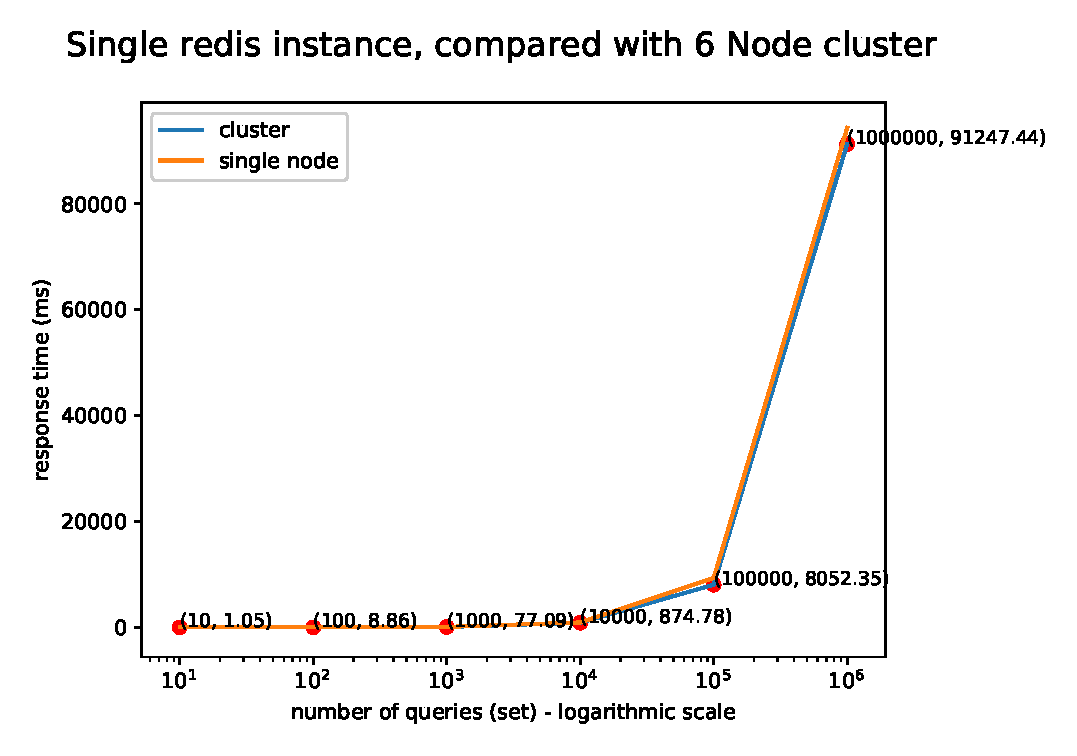
\includegraphics[width=\textwidth]{fig5.eps}
\end{frame}
    
\begin{frame}
    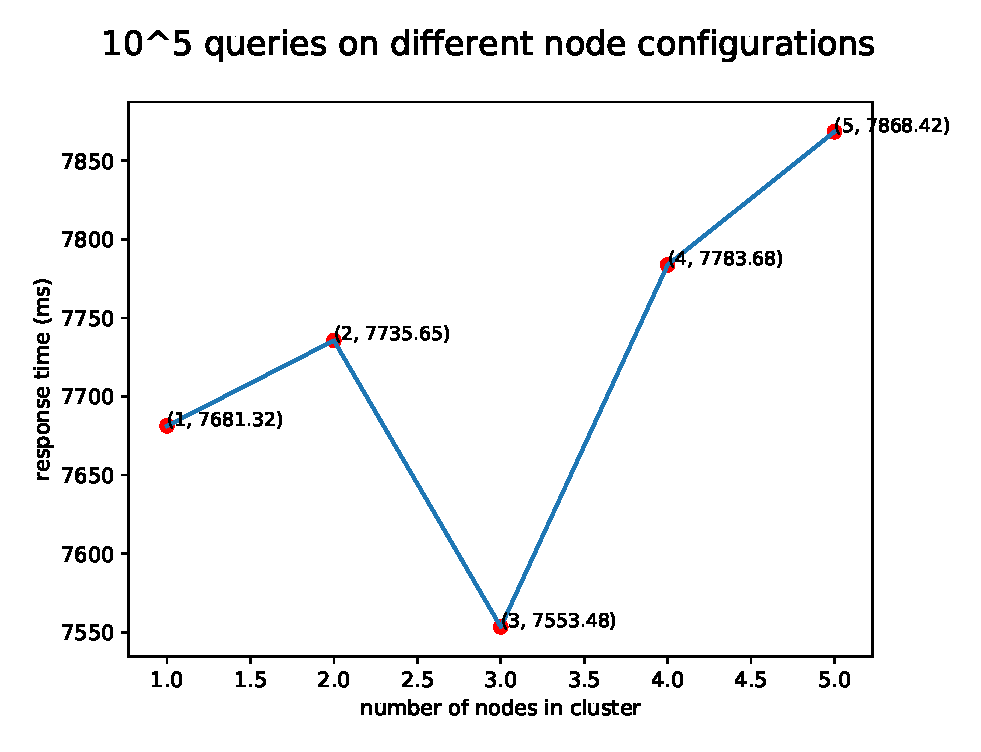
\includegraphics[width=\textwidth]{fig6.eps}
\end{frame}

\begin{frame}
    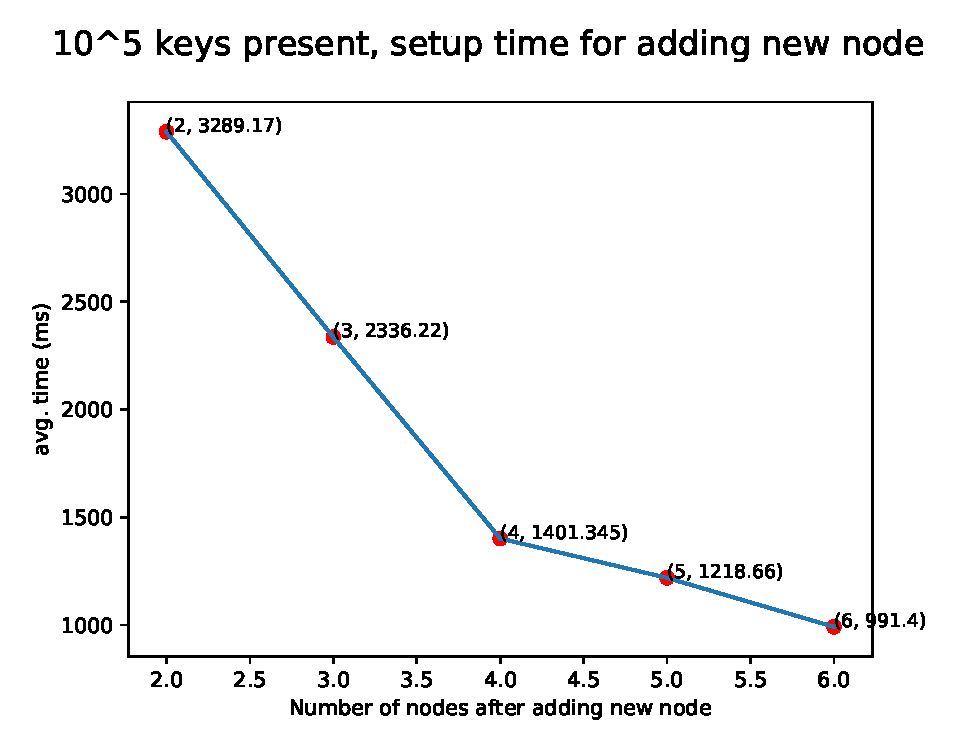
\includegraphics[width=\textwidth]{fig7.eps}
\end{frame}

\begin{frame}
    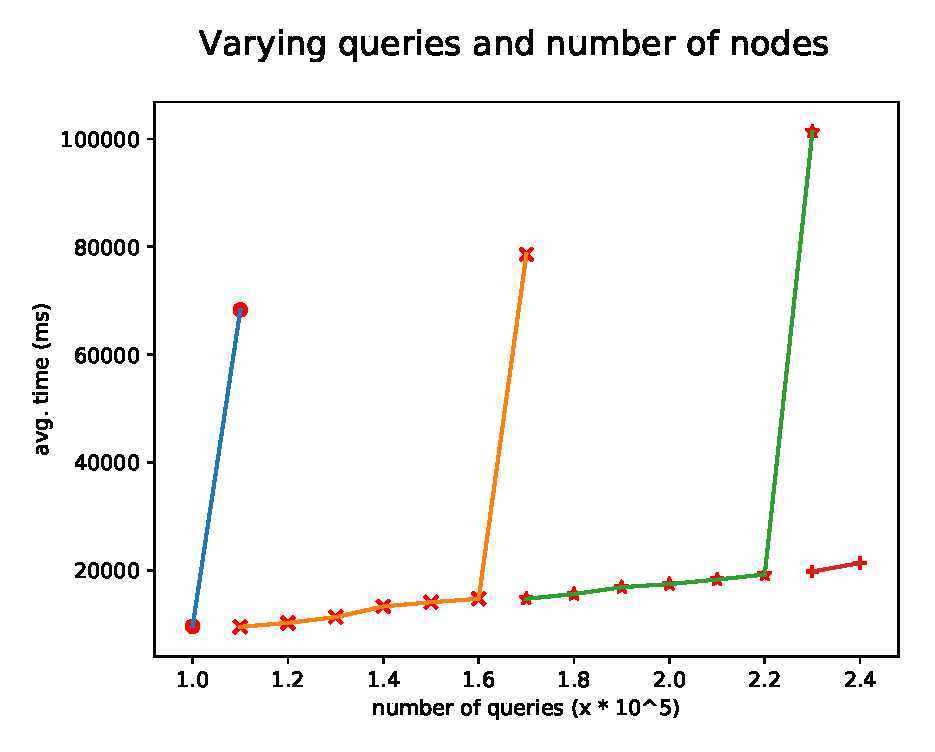
\includegraphics[width=\textwidth]{fig8.eps}
\end{frame}

\section{Current Picture}

\begin{frame}{Machine Learning based solutions}
\begin{itemize}
    \pause\item \textit{Auto-Scaling Network Resources using Machine Learning to Improve QoS and Reduce Cost} arxiv-1808.02975
    \pause\item Measured network traffic load to dynamically react to traffic changes.
    \pause\item A classification problem.
    \pause\item This ML classifier learns from past network scaling decisions and seasonal/spatial
            behavior of network traffic load to generate scaling decisions ahead of time. 
    \pause\item Models used:
        \begin{itemize}
                \pause\item Reduced Error Pruning Tree.
                \pause\item Decision Table.
                \pause\item Multi-Layer Perceptron.
                \pause\item DNNs.
        \end{itemize}
    \pause\item Features used :=  startup time, resource utilization factor, etc.
\end{itemize}
\end{frame}

\begin{frame}{Static metric based approach}
    \begin{itemize}
        \pause\item \textit{Containers Orchestration with Cost-Efficient Autoscaling in Cloud Computing Environments - arxiv:1812.00300}
        \pause\item Simple Autoscaler.
            \begin{itemize}
                \pause\item elapsed time since last instance launched $>=$ provisioning\_interval
            \end{itemize}
        \pause\item Single Instance Binding Autoscaler.
            \begin{itemize}
                \pause\item multiple requests to autoscale triggered by the same unschedulable pod may be invoked.
            \end{itemize}
    \end{itemize}
\end{frame}

\begin{frame}{Performace models}
    \begin{itemize}
        \pause\item \textit{Automatic configuration and scaling of stream processing pipelines - arxiv:1812.09442}
        \pause\item precise performance models can be automatically
learned for distributed stream processing systems
that can predict the execution performance of a job
even before deployment.
    \pause\item These models can be
used to optimally schedule logically specified jobs onto
available physical hardware.

    \pause\item These models and
the derived execution schedules can be refined online to
dynamically adapt to unpredictable changes in the runtime
environment or auto-scale with variations in job
load.
    \end{itemize}
\end{frame}


\section{Further works}
\begin{frame}{Further Works}
    \begin{itemize}
        \pause\item Implement dynamic scaling feature in twemproxy.
        \pause\item Add a service on top of twemproxy to apply scaling logic (based on statistics recieved from twem).

        \pause\item Test some state of the art machine learning algorithms like Meta learning, Siamese nets etc.
    \end{itemize}
\end{frame}

\begin{frame}
    \begin{center}
    \Huge{Thank You!}
    \end{center}
    \end{frame}



\end{document}
